\documentclass[aspectratio=169,compress]{beamer}
%---------------------------------------------> Comando para deixar justificado 
%                                               o texto nos blocos: \justifying
%
%==============================================================================
% Pacotes
%==============================================================================
\ProvidesPackage{sty/beamercolorthemeNord}
\ProvidesPackage{sty/beamerfontthemeNord}
\ProvidesPackage{sty/beamerthemeNord}

\usepackage{fontspec}
\usepackage{polyglossia}
 \setdefaultlanguage[variant=brazilian]{portuguese}
\usepackage{amsmath, amssymb, amsfonts, amscd}
 \usefonttheme[onlymath]{serif}
\usepackage{ragged2e}%----------------------> Paragrafo justificado \justifying
\usepackage{esint}%-------------------> Integrais circulares  \ointctrclockwise
\usepackage{array}
\usepackage{graphicx}
 \graphicspath{{./figs/}}
\usepackage{metalogo}
\usepackage{booktabs}
\usepackage{listings}
\usepackage{tikz}
%==============================================================================

%==============================================================================
% Configurações do Beamer
%==============================================================================
\usetheme{Nord}
%------------------------------------------------------------------------------
\AtBeginSection[]
{
  \begin{frame}[c,noframenumbering,plain]
    \tableofcontents[sectionstyle=show/hide,subsectionstyle=show/show/hide]
  \end{frame}
}

\AtBeginSubsection[]
{
  \begin{frame}[c,noframenumbering,plain]
    \tableofcontents[sectionstyle=show/hide,subsectionstyle=show/shaded/hide]
  \end{frame}
}
%------------------------------------------------------------------------------
%==============================================================================

%==============================================================================
% Novos Comandos
%==============================================================================
% Operadores ------------------------------------------------------------------
% \DeclareMathOperator{\nec}{nec}
%------------------------------------------------------------------------------
% Comandos --------------------------------------------------------------------
\newcommand{\cqd}{\hfill $\blacksquare$}
%------------------------------------------------------------------------------
%==============================================================================


%------------------------------------------------------------------------------
% Titulo
%------------------------------------------------------------------------------
\title{A Ação Divina no Mundo}
\subtitle{As Perspectivas Antigas}
\author{Ícaro, Jacqueline \& Lucas }
\institute{Contraponto/CFP/UFRB}
\date{\today}
%------------------------------------------------------------------------------
 %------> Preâmbulo tex

\newcommand{\V}{\textbf{V}}
\newcommand{\F}{\textbf{F}}
%================================================
% Inicio do Documento
%================================================
\begin{document}
%------------------------------------------------
\begin{frame}[plain,noframenumbering]
 \maketitle
\end{frame}
\section{Introdução}

\begin{frame}{Esclarecimentos Iniciais}
 \centering
 \includegraphics<2->[width = 0.5\textwidth]{chess}
 
 \begin{minipage}{0.8\textwidth}
  \begin{exampleblock}<3->{\textbf{Possível Conflito}}
   \justifying
    As ações de Deus no mundo (os milagres) são incompatíveis com a ciência
    contemporânea.
  \end{exampleblock}
 \end{minipage} 
\end{frame}

\begin{frame}<1-11>[label=mundos]{Esclarecimentos Iniciais}{O que pensa o Cristão?} %-----> marcação para esclarecimentos
 \begin{itemize}
  \item<2-|alert@2> Deus é uma Pessoa;
   \only<3-5>{
    \begin{itemize}
     \item<3-5> ser dotado de conhecimento e afeição;
     \item<4-5> ser com objetivos definidos;
     \item<5> age para alcançar tais objetivos.
    \end{itemize}
   }
  \item<6-|alert@6> Deus é Onisciente, Onipotente, Onipresente e Completamente Bom;
  \item<7-|alert@7> Deus é um ser necessário;
   \only<8-13>{
    \begin{itemize}
     \item<8-> existe em todos os ``mundos possíveis''
      \begin{itemize}
       \item<9-> alternativas que Deus tinha para criar o mundo (Leibniz)
       \item<10-> formas como as coisas poderiam ter sido, se elas fossem diferentes.
       \item<11-> descrição consistente da realidade
      \end{itemize}
     \item<12-> Verdades Necessárias
      \begin{itemize}
       \item<13> verdades em todos os mundos possíveis.
      \end{itemize}
    \end{itemize}
   }
  \item<14-|alert@14> Deus criou o mundo;
  \item<15-|alert@15> Deus conserva o mundo;
   \only<16-18>{
    \begin{itemize}
     \item<16-> alguns veem como ``recriação'';
     \item<17-> \textcolor{NordYellow}{convir} de Deus e o mundo
      \begin{itemize}
       \item<18-> Deus ``permite'' toda ocorrência causal
      \end{itemize}
    \end{itemize}
   }
  \item<19-|alert@19> Nada é ``mero acaso''.
   \begin{itemize}
    \item<20-> há regularidade e previsibilidade
    \item<21-> Deus, às vezes, age de forma diferente (trata diferente sua criação)
     \begin{itemize}
      \item<22-> \textcolor{NordYellow}{ação particular} (vai além da criação e conservação.)
     \end{itemize}
   \end{itemize}
 \end{itemize}

\end{frame}

\begin{frame}{\textbf{Mundos possível?}}
  \begin{exampleblock}{Em termos proposicionais}
   \begin{itemize}
    \item<2-> Nosso mundo (mundo real):
     \only<3->{
      \[
       p_1 \wedge p_2 \wedge p_3 \wedge \ldots \wedge p_n ;
      \]
     }
    \item<4-> Outros mundos: qualquer combinação que negue o mundo real.
      \begin{align*}
       \only<5->{\textcolor{NordYellow}{(\sim\! p_1)} \wedge p_2 \wedge p_3 \wedge &\ldots \wedge p_{n-1}\wedge p_n\\}
       \only<6->{p_1 \wedge \textcolor{NordYellow}{(\sim\! p_2)} \wedge p_3 \wedge &\ldots \wedge p_{n-1}\wedge p_n\\}
       \only<7->{p_1 \wedge p_2 \wedge \textcolor{NordYellow}{(\sim\! p_3)} \wedge &\ldots \wedge p_{n-1}\wedge p_n\\}
       \only<8->{&\;\;\vdots}
      \end{align*}
   \end{itemize}
  \end{exampleblock}
\end{frame}

\begin{frame}{Mundos possíveis?}
	 \begin{exampleblock}{Exemplos possíveis}
   \begin{itemize}[<+->]
    \item Mundo real:     \textcolor{NordYellow}{Asaph não caiu da \textit{bike} descendo a ladeira.}
    \item Mundo Possível: \textcolor{NordYellow}{Asaph caiu da \textit{bike} a ladeira.}
    \item Mundo real:     \textcolor{NordGreen}{Glênon é um professor carrasco de física.}
    \item Mundo possível: \textcolor{NordGreen}{Glênon não é um professor carrasco de física.}
    \item Mundo real:     \textcolor{NordYellow}{Cachorros não falam ou escrevem}
    \item Mundo possível: \textcolor{NordYellow}{Cachorros falam e escrevem}
    \item Mundo real:     \textcolor{NordGreen}{Agora está chovendo.}
    \item Mundo Possível: \textcolor{NordGreen}{Agora não está chovendo.}
   \end{itemize}
  \end{exampleblock}
  
  \begin{block}<9->{Pergunta importante}
   \only<10->{$\triangleright$ É possível, em qualquer mundo, está chovendo e não chovendo?}
  \end{block}
\end{frame}

\begin{frame}{Falsidades Necessárias}
	 \begin{exampleblock}<2->{Exemplos de falsidades em qualquer mundo possível}
   \begin{itemize}
    \item<3-> $ p \wedge (\sim\! p)$;
    \item<4-> A ideia de que ``$ 1 + 1 \neq 2 $''.
    \item<5-> Um objeto que possui qualidades maximais em certo conjunto, mas que não contenha alguma qualidade desse conjunto.
   \end{itemize}
  \end{exampleblock}
  
  \begin{itemize}
   \item<6-> Qual o contrário de Falsidades Necessárias?
    \begin{itemize}
     \item<7-> Tautologias $\big(\text{e.g.: } p \vee (\sim\! p)\big)$: Está chovendo ou não chovendo.
     \item<8-> A ideia de que ``$ 1 + 1 = 2 $''
    \end{itemize}
   \item<9-|alert@9> É possível um ser maximal existir em um mundo possível e não existir em outro?
   \item<10-> Falsidades Necessárias \textit{vs} \textcolor{NordGreen}{Verdades Necessárias}
  \end{itemize}
\end{frame}

\againframe<12->{mundos} %----------------> volta à marcação do frame principal
\section{O (suposto) Problema}

\begin{frame}{Teólogos que veem problema}
\begin{columns}
\begin{column}{0.7\textwidth}
	 \begin{itemize}
			 \item<2->[$\bullet$] \textcolor{NordBrightCyan}{\textbf{Gilkey}}: teólogos não acreditam que Deus 
				 tenha realizado milagres!
				 \begin{itemize}
					 \item<5-> a Bíblia é um livro de interpretação
					 \item<6-> dizer $\times$ crer
				 \end{itemize}
			 \item<3->[$\bullet$] \textcolor{NordBrightCyan}{\textbf{Bultmann}}: Deus não age no mundo!
			  \begin{itemize}
					 \item<7-> a história é uma \textcolor{NordYellow}{sequência fechada de efeitos}.
					 \item<8-> não pode sofrer intervenções de poderes sobrenaturais
					 \item<9-> causa e efeito
					 \item<10-> Lei dos Medos e Persas
				 \end{itemize}
			 \item<4->[$\bullet$] \textcolor{NordBrightCyan}{\textbf{Macquarrie}}: rompimento da ordem natural
			  \begin{itemize}
					 \item<11-> ciência e história são \textbf{\textcolor{NordRed}{inconciliáveis}}
					  com a ideia de ``milagres''.
					 \item<12-> motivo: causa e efeito
					  \begin{itemize}
					   \item<13->[-] conhecimento limitado apenas temporariamente.
						\end{itemize}
				\end{itemize}
		\end{itemize}
\end{column}
\begin{column}{0.3\textwidth}
 \only<2, 5-6>{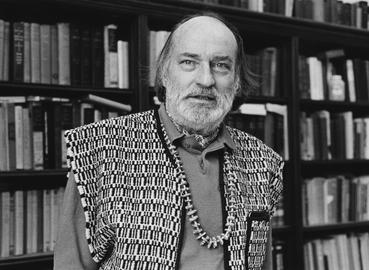
\includegraphics[width = 4cm]{gilkey}}
	\only<3, 7-10>{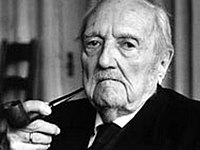
\includegraphics[width = 4cm]{bultmann}}
	\only<4, 11-13>{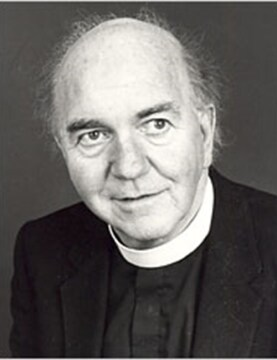
\includegraphics[width = 4cm]{macquarrie}}
\end{column}
\end{columns}
\end{frame}

\begin{frame}{Teólogos que veem problema}
\centering
\begin{minipage}{\textwidth}
	\begin{exampleblock}{\textbf{Observações}}
	 \begin{itemize}
			\item<2->[$\bullet$] Bultmann e Macquarrie acham compatíveis a ``ação geral'' de Deus 
			 (preservação da existência do mundo), mas não a ``ação particular'';
			\item<3->[$\bullet$] A ação particular é um problema porque: é incompatível com a ciência
			 moderna.
				\begin{itemize}
					\item<4-> a ciência \textcolor{NordYellow}{demonstra} ou 
					 \textcolor{NordYellow}{pressupõe} que Deus não age assim;
					\item<5-> a ciência é a Razão.
				\end{itemize}
		\end{itemize}
	\end{exampleblock}
	\end{minipage}
\end{frame}

\begin{frame}{Filósofo ou Cientistas que veem problema}
 \begin{columns}
	 \begin{column}{0.45\textwidth}
	  \begin{itemize}
			 \justifying
		  \item<2-3,8-14>[$\bullet$] \textcolor{NordBrightCyan}{Philip Clayton}: a ciência 
				 tem a capacidade de explicar e prever os fenômenos naturais.
	  \end{itemize}
			\vspace{0.5cm}
			\centering
			\only<2-3, 8-14>{
\includegraphics[width = 4cm]{clayton}}
			\only<4>{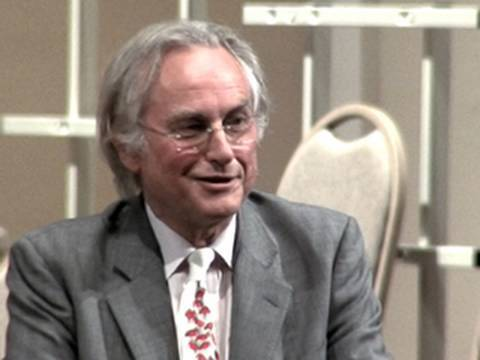
\includegraphics[width = 4cm]{dawkins}}
			\only<5>{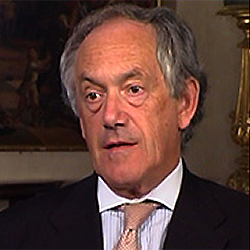
\includegraphics[width = 4cm]{peter}}
			\only<7>{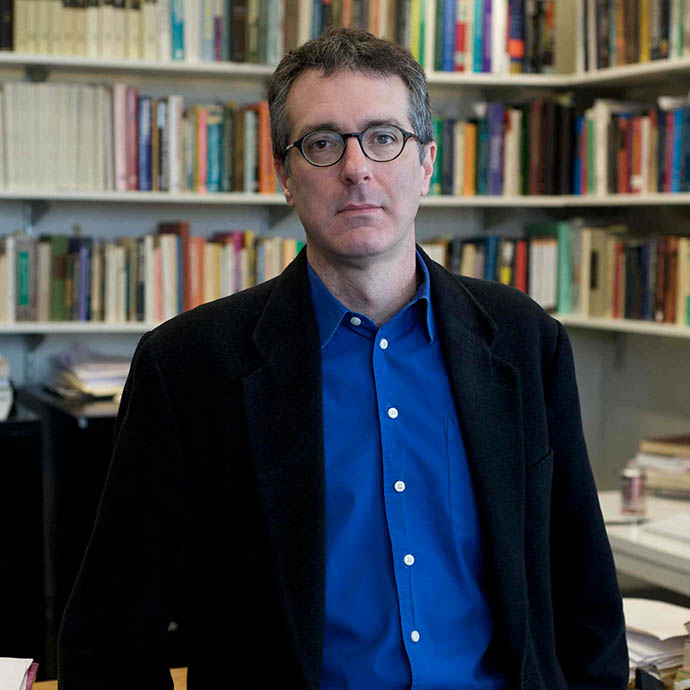
\includegraphics[width = 4cm]{orr}}
			\only<6>{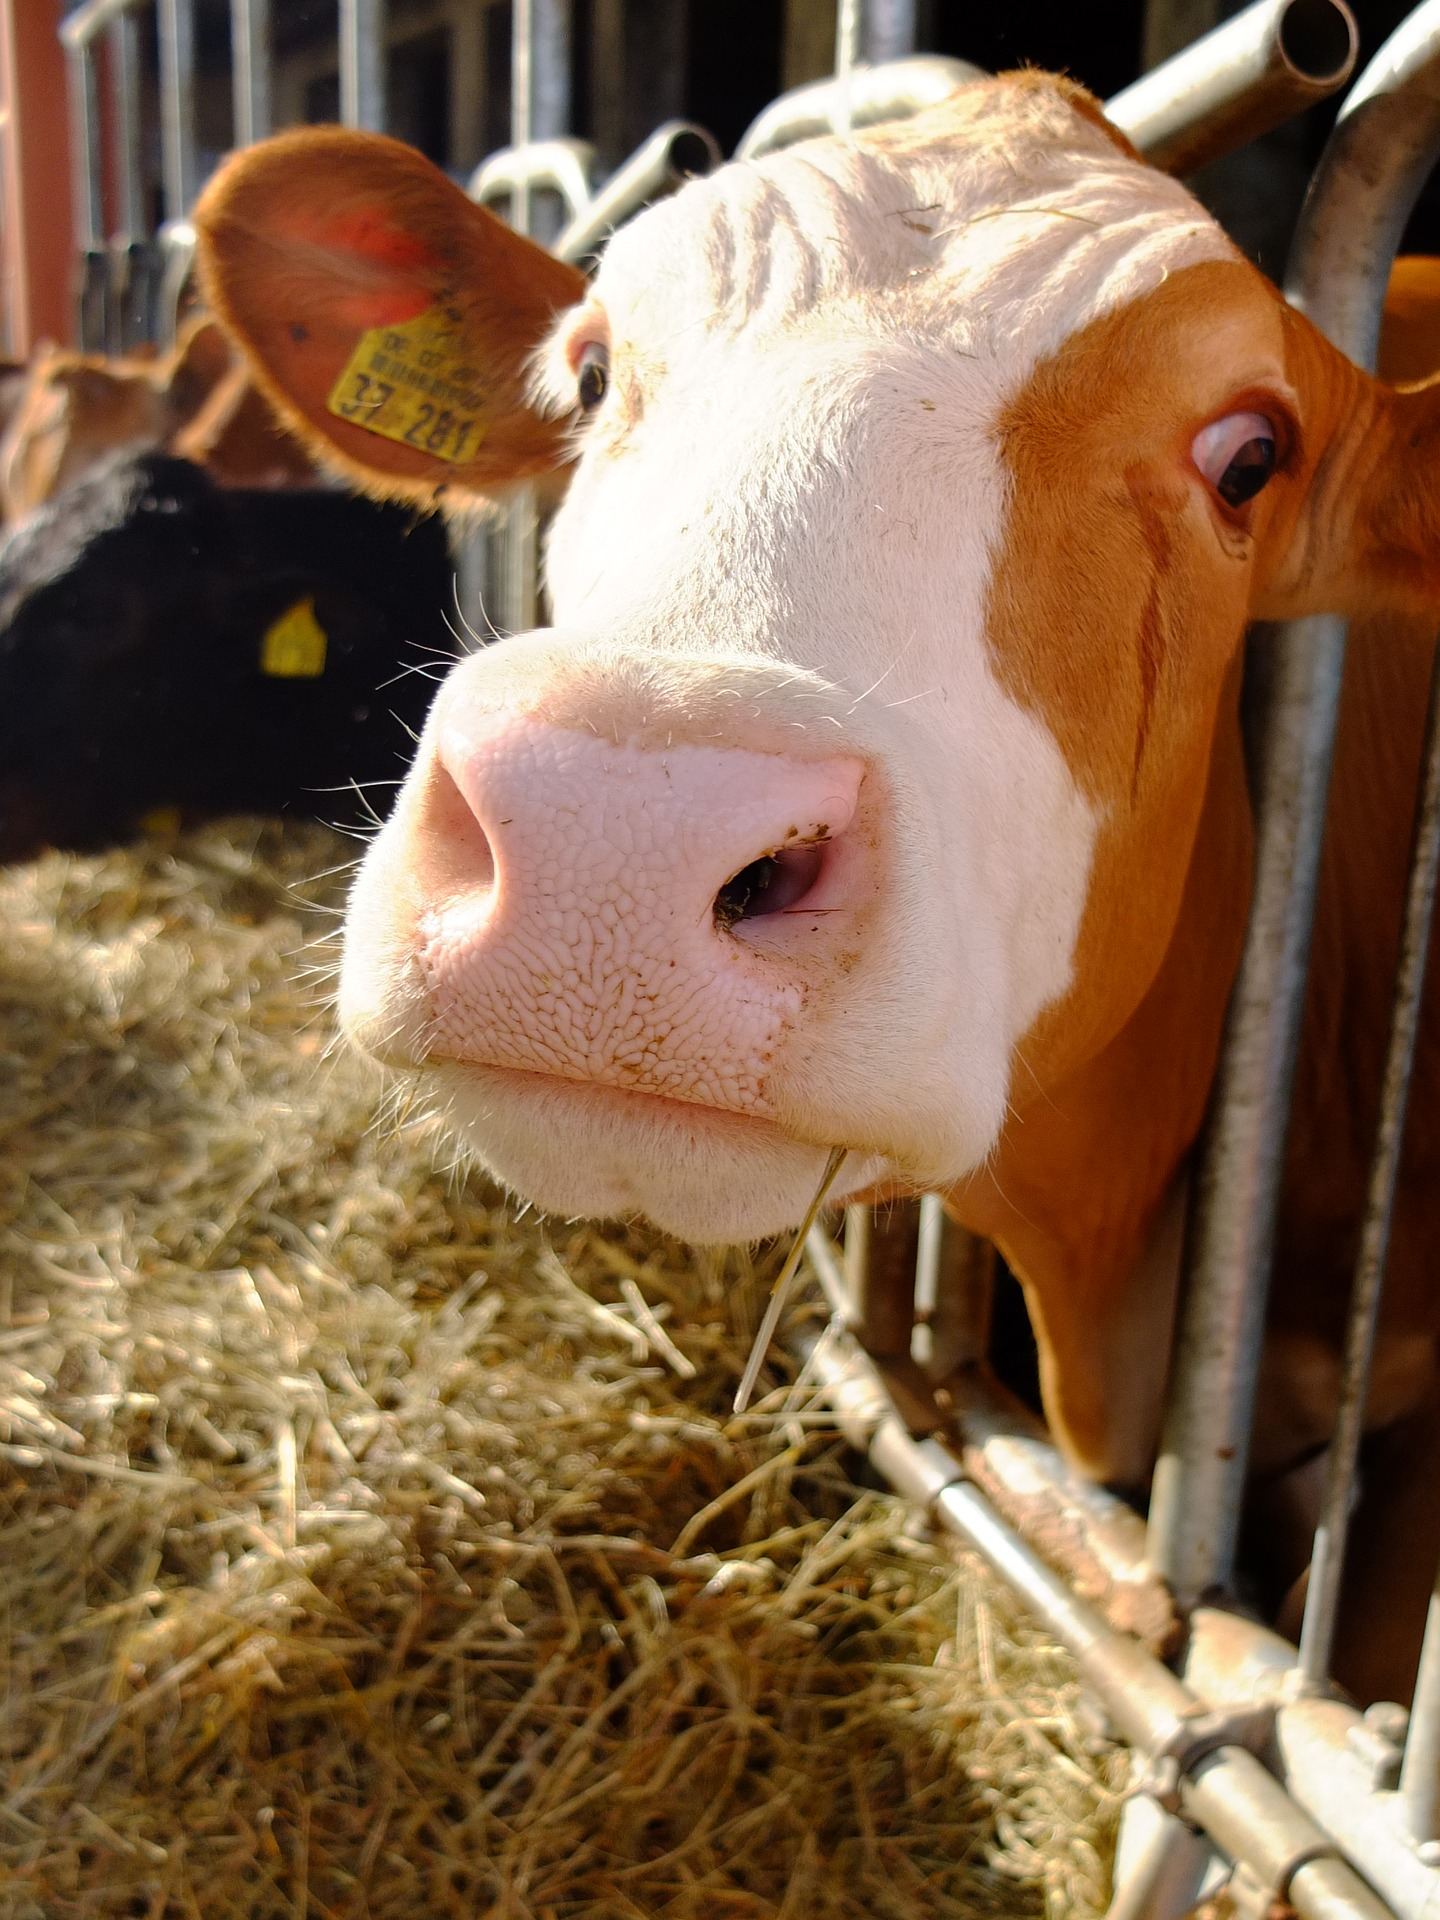
\includegraphics[width = 4cm]{vaca}}
			\only<15>{
\includegraphics[width = 4cm]{merovingian}}
			\only<16>{
\includegraphics[width = 4cm]{sherlock}}
			\only<17>{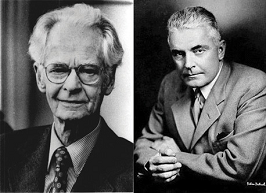
\includegraphics[width = 4cm]{watson-skinner}}
		\end{column}
		\begin{column}{0.55\textwidth}
		 \begin{itemize}
			 \item<3-> Cientitas com Clayton: 
				 \begin{itemize}
					 \item<4-> \onslide<4->{Richard Dawkins}\onslide<5->{, Peter Atkins} \onslide<6->{(loucos?)}
					 \item<7-> H. Allen Orr (sensato)
					\end{itemize}
				\item<8-|alert@8> Ciência $\Longleftrightarrow$ \textcolor{NordYellow}{Determinismo}
					\begin{itemize}
						\item<9-> Exclusão de Deus (ação particular)
						\item<10-> At 17.18: estóicos \textit{vs} epicureus
							\begin{itemize}
								\item<11-> virtude: reação diante do determinismo materialista
								\item<12-> o ser humano não pode determinar seu destino
								\item<13-> ataraxia
								\item<14-> Síndrome de Gabriela
							\end{itemize}
						\item<15-> Filme Matrix
						\item<16-> Sherlock Holmes
						\item<17-> Skinner e Watson
					\end{itemize}
			\end{itemize}
		\end{column}
	\end{columns}
\end{frame}

\begin{frame}{Um dos Perigos do Determinismo}
 \begin{quote}
		\onslide<2->{Nossos membros estão praticamente sempre fazendo o que 
		\textcolor{NordOrange}{querem} fazer --- o que eles 
		\textcolor{NordOrange}{escolhem} fazer --- mas nós cuidamos para que eles 
		queiram fazer precisamente as coisas	que são melhores para eles e para a 
		comunidade.}
		\onslide<3->{Seu comportamento é determinado, ainda que eles sejam livres.}
		\onslide<4->{Ditadura e liberdade, determinismo e livre-arbítrio.}
		\onslide<5->{O que é isso senão pseudoquestões de origem linguística?}
		\onslide<6->{Quando perguntamos o que o Homem pode fazer do Homem, nós não 
		queremos dizer	a mesma coisa por ``homem'' em ambos os casos.}
		\onslide<7->{Queremos perguntar o que alguns poucos homens podem fazer da 
		humanidade.}
		\onslide<8->{E essa é a questão central do século XX.} 
		\onslide<9->{Que tipo de mundo podemos construir --- nós que entendemos a 
		ciência do comportamento?} \onslide<10->{(\textcolor{NordYellow}{Skinner})}
	\end{quote}
\end{frame}

\begin{frame}{\textbf{Resumo do Problema}}
	\centering
			\begin{minipage}{\textwidth}
			\begin{exampleblock}{\textbf{Resumo do ``Problema''}}
			 \begin{enumerate}[(1)]
					\item<2-> A Ciência descobre e endossa Leis Naturais;
					\item<3-> As ações particulares de Deus violaria as Leis Naturais;
					\item<4-> Isso é incompatível com a Ciência.
				\end{enumerate}
			\end{exampleblock}
			\end{minipage}
\end{frame}
\section{Perspectivas Antigas}

%------------------------------------------------------------------------------
\subsection{Panorama}
%------------------------------------------------------------------------------
\begin{frame}{\textbf{Panorama}}
	\begin{itemize}
		\item<2->[$\bullet$] Tal conflito deriva de uma \textcolor{NordRed}{concepção 
		 particular da ciência clássica.}
			\begin{itemize}
				\only<3>{\item \textit{Weltanshauung}: visão de mundo}
				\item<4-> mecânica newtoniana
				\item<5-> física da eletricidade e magnetismo
				 \begin{itemize}
						\item<6->[-] conservação do momento (3ª Lei de Newton)
						\item<7->[-] conservação da energia
					\end{itemize}
			\end{itemize}
	\end{itemize}
\end{frame}


%------------------------------------------------------------------------------
\subsection{A perspectiva newtoniana}
%------------------------------------------------------------------------------
\begin{frame}{\textbf{A perspectiva newtoniana}}

	 \centering
	 \begin{minipage}{\textwidth}
	  \begin{exampleblock}<2->{O que diz?}
		  O Universo material é uma imensa máquina que evolui ou opera de acordo com
			 \textcolor{NordYellow}{leis fixas} (leis da Física Clássica)
		 \end{exampleblock}
	 \end{minipage}
	
	\vspace{0.5cm}
	\begin{itemize}
		\item<3->[$\bullet$] As leis refletem a natureza das coisas
		\item<4->[$\bullet$] Podem ser decretos de Deus para o comportamento da matéria
		\item<5->[$\bullet$] Todo mundo mecânico poderia ser reduzido às leis físicas
		 \begin{itemize}
				\item<6-> inclusive Leis da Biologia ou da Química
				\item<7-> \textcolor{NordRed}{completude da física clássica}: um acréscimo
					filosófico
			\end{itemize}
	\end{itemize}
\end{frame}

\begin{frame}{\textbf{A perspectiva newtoniana}}
 \begin{itemize}
		\item<2->[$\bullet$] \onslide<2->{Perspectiva newtoniana} \onslide<3->{$\not\Rightarrow$} 
		 \onslide<4->{\textcolor{NordYellow}{teologia da não interferência divina}}
			\begin{itemize}
				\item<5-> Newton aceitava a interferência divina: ajustes das órbitas dos planetas
				\item<6-> As Leis Naturais descrevem o funcionamento do mundo 
				 ``desde que o mundo seja um \textcolor{NordRed}{sistema fechado} (isolado) 
					não sujeito a nenhuma influência causal exterior''
					\begin{itemize}
						\item<7->[-] as grandes leis seguem esse princípio (sistema isolado) 
					\end{itemize}
				\item<8-> Quem estabeleceu que o mundo é ``fechado''?
				 \begin{itemize}
						\item<9->[-] se o sistema \textcolor{NordOrange}{não} é fechado, não há 
							problema da \textcolor{NordOrange}{ação particular} de Deus.
					\end{itemize}
			\end{itemize}
			
			\centering
			\begin{minipage}{\textwidth}
			\begin{block}<10->{Diferença Crucial}
			\centering
			 \onslide<11->{\textcolor{NordBrightCyan}{Dizer como as coisas são sempre}}\\
					\onslide<12->{$\neq$}\\ 
				\onslide<13->{\textcolor{NordCyan}{Dizer como as coisas são quando nenhum agente 
					exterior ao universo age.}}
			\end{block}
			\end{minipage}
	\end{itemize}
	
\end{frame}

\begin{frame}{\textbf{A perspectiva newtoniana}}
	\begin{exampleblock}{Relembrando Lógica\ldots}
	 \begin{itemize}
			\item[$\bullet$] Tabela Verdade da Conjunção, Disjunção e Condicional\\
			 \begin{center}
				\only<2-10>{
				\begin{tabular}{ccccc}
				 \toprule
				 $p$ & $q$ & $p \wedge q$ & $p \vee q$ & \only<3->{\textcolor{NordYellow}{$p \rightarrow q$}}\\
					\midrule
					\V  & \V  & \V           & \V         & \only<5->{\textcolor{NordYellow}{\V}}\\
					\V	 & \F  & \V           & \V         & \only<4->{\textcolor{NordOrange}{\F}}\\
					\F  & \V  & \F           & \V         & \only<5->{\textcolor{NordYellow}{\V}}\\
					\F  & \F  & \F           & \F         & \only<5->{\textcolor{NordYellow}{\V}}\\
					\bottomrule
				\end{tabular}
				}
				\only<11->{
				\begin{tabular}{ccccccc}
				 \toprule
				 $p$ & $q$ & $p \wedge q$ & $p \vee q$ & \textcolor{NordYellow}{$p \rightarrow q$} & \only<12->{$\sim\! p$ & \only<14->{\textcolor{NordYellow}{$\sim\! p \vee q$}}} \\
					\midrule
					\V  & \V  & \V           & \V         & \textcolor{NordYellow}{\V} & \only<13->{\F} &\only<16->{\textcolor{NordYellow}{\V}}\\
					\V	 & \F  & \V           & \V         & \textcolor{NordOrange}{\F} & \only<13->{\F} &\only<15->{\textcolor{NordOrange}{\F}}\\
					\F  & \V  & \F           & \V         & \textcolor{NordYellow}{\V} & \only<13->{\V} &\only<16->{\textcolor{NordYellow}{\V}}\\
					\F  & \F  & \F           & \F         & \textcolor{NordYellow}{\V} & \only<13->{\V} &\only<16->{\textcolor{NordYellow}{\V}}\\
					\bottomrule
				\end{tabular}
				}
				\end{center}
			\item<1, 6->[$\bullet$] Equivalências Lógicas
				\begin{itemize}
					\item<7-> $ p \wedge (q\vee r) \Leftrightarrow (p\wedge q) \vee (p\wedge r) $
					\item<8-9,10-> \only<8-9>{$ p\rightarrow q \Leftrightarrow\, \sim\! p \vee q $} \only<10->{\textcolor{NordYellow}{$ p\rightarrow q \Leftrightarrow\, \sim\! p \vee q $}}
					\item<9-> $ (p \vee q) \rightarrow r \Leftrightarrow (p\rightarrow r) \wedge (q\rightarrow r)$
				\end{itemize}
		\end{itemize}
	\end{exampleblock}
\end{frame}

\begin{frame}{\textbf{Determinismo necessariamente verdadeiro?}}
	\begin{description}
	 \item<2->[$u$:] universo é casualmente fechado
		\item<3->[$p$:] consequentes de todas as leis
		\item<4->[$\ell$:] passado
		\item<5->[$f$:] futuro
		\item<6->[$\square$:] operador ``necessidade''
	\end{description}
	\centering
	\begin{minipage}{\textwidth}
  \begin{exampleblock}<7->{Definições}
	  \begin{itemize}
		  \item<8-> \textcolor{NordYellow}{Lei Natural}: \only<9->{$u\rightarrow p$}
			 \item<10-> \textcolor{NordYellow}{Determinismo}: \only<11->{$[(u\rightarrow p) \wedge \ell]\rightarrow f$}
			 \item<12-> \textcolor{NordYellow}{Determinismo Necessariamente Verdadeir}: \only<13->{$\square\left\{\,[(u\rightarrow p) \wedge \ell]\rightarrow f\,\right\}$}
		 \end{itemize}
	 \end{exampleblock}
	\end{minipage}
\end{frame}

\begin{frame}{\textbf{Demonstração}}
\onslide<2->{Suponha o Determinismo \textcolor{NordCyan}{necessariamente} verdadeiro.}
\onslide<3->{Então,}
\only<4->{
 \begin{align*}
	 \only<4->{\square\left\{\,[(u\rightarrow p) \wedge \ell]\rightarrow f\,\right\}} 
		\only<5->{&\Leftrightarrow}
		\only<6->{\square\left\{\,[\textcolor{NordRed}{(\sim\! u \vee p)} \wedge \ell]\rightarrow f\,\right\}}\\
		\only<7->{&\Leftrightarrow
		\square\left\{\,[\ell \wedge \textcolor{NordRed}{(\sim\! u \vee p)}]\rightarrow f\,\right\}}\\
		\only<8->{&\Leftrightarrow}
		\only<9->{\square\left\{\,[\only<10->{\textcolor{NordYellow}{(\ell \wedge \sim\! u)}} \only<11->{\vee} \only<12->{\textcolor{NordOrange}{(\ell \wedge p)}}]\rightarrow f\,\right\}}\\
		\only<13->{&\Leftrightarrow}
		\only<14->{\square\left\{\,\textcolor{NordYellow}{(\ell \wedge \sim\! u)}\rightarrow f\,\right\}} \only<15->{\quad\wedge\quad} \only<16->{\square\left\{\,\textcolor{NordOrange}{(\ell \wedge p)}\rightarrow f\,\right\}}
	\end{align*}
}
	
	\begin{itemize}
		\item<17->[$\bullet$] $(\ell \wedge \sim\! u ) \rightarrow f$ é falso, pois:
		 \begin{itemize}
				\item<18-|alert@18> existe um mundo possível com o mesmo passado que o nosso: $\ell$;
				\item<19-|alert@19> não seja fechado: $\sim\! u$;
				\item<20-|alert@20> mas, não possui o mesmo futuro: $\sim\! f$.
			\end{itemize}
		\item<21->[$\bullet$] Como $(\ell \wedge \sim\! u) \rightarrow f$ é falso, então
			$[(u\rightarrow p) \wedge \ell]\rightarrow f$ é necessariamente falso.
			O que é uma contradição!
		\item<22-> A contradição veio do fato de supormos o Determinismo necessariamente
		verdadeiro.
	\end{itemize}
\end{frame}

\begin{frame}{A perspectiva newtoniana}
 \centering
	\begin{minipage}{\textwidth}
 \begin{exampleblock}{Resumo\ldots}
	 \begin{itemize}[<+->]
			\item Não  há ``violação'' de lei; pois, ao agir Deus, o sistema não é mais
				fechado;
			\item Não cabe a ciência clássica afirmar que as leis não podem ser violadas;
			\item Portanto,
			\begin{align*}
				\only<4->{\text{Ciência Clássica } &\not\Rightarrow \textcolor{NordYellow}{ Determinismo}}\\
				\only<5->{&\text{ ou}}\\
				\only<6->{\text{Ciência Clássica } &\not\Rightarrow \textcolor{NordYellow}{ Universo casualmente fechado}}
			\end{align*}
		\end{itemize}
	\end{exampleblock}
	\end{minipage}
\end{frame}

%------------------------------------------------------------------------------
\subsection{A perspectiva laplaciana}
%------------------------------------------------------------------------------
\begin{frame}{\textbf{A perspectiva laplaciana}}
	\begin{itemize}
		\item<2->[$\bullet$] A perspectiva laplaciana orienta o pensamento dos teólogos da
		 não interferência divina.
		\item<3->[$\bullet$] $\only<4->{\text{Perspectiva laplaciana }} \only<5->{=} \only<6->{\text{ newtoniana }} \only<7->{+} \only<8->{\text{ fecho causal do universo.}} $
		 \begin{itemize}
				\item<9-> \textcolor{NordRed}{acréscimo filosófico}
				\item<10-> a ciência clássica não atesta que o ``universo é fechado''
			\end{itemize}
		\item<11->[$\bullet$] $\text{não poder agir } \neq \underbrace{\text{ não agir na prática}}_{\text{perspectiva laplaciana}} $
		\item<12->[$\bullet$] Consequências para a Liberdade Humana
		 \begin{itemize}
				\item<13-> nenhuma ação humana é livre
			\end{itemize}
	\end{itemize}
	\centering
	\begin{minipage}{\textwidth}
	 \begin{exampleblock}<14->{Conclusão\ldots}
		 Não há conflito entre Ciência e Religião!
			\only<15->{O conflito existe entre a Religião e uma metafísica particular, na qual 
			afirma que o universo é causalmente fechado.}
		\end{exampleblock}
	\end{minipage}
\end{frame}

%------------------------------------------------
\end{document}
%================================================